% --------------------------------------------------------------
% This is all preamble stuff that you don't have to worry about.
% Head down to where it says "Start here"
% --------------------------------------------------------------
 
\documentclass[12pt]{article}
 
\usepackage[margin=1in]{geometry} 
\usepackage{amsmath,amsthm,amssymb}
\usepackage{graphicx, float}
\usepackage{listings}
\usepackage{CJKutf8}
\usepackage{physics}
 
\newcommand{\N}{\mathbb{N}}
\newcommand{\Z}{\mathbb{Z}}

\newcommand{\e}{\epsilon}
\newcommand{\yn}{\y_n}
\newcommand{\xn}{\x_n}
\newcommand{\wT}{\w^T}
 
\newenvironment{theorem}[2][Theorem]{\begin{trivlist}
\item[\hskip \labelsep {\bfseries #1}\hskip \labelsep {\bfseries #2.}]}{\end{trivlist}}
\newenvironment{lemma}[2][Lemma]{\begin{trivlist}
\item[\hskip \labelsep {\bfseries #1}\hskip \labelsep {\bfseries #2.}]}{\end{trivlist}}
\newenvironment{exercise}[2][ ]{\begin{trivlist}
\item[\hskip \labelsep {\bfseries #1}\hskip \labelsep {\bfseries #2.}]}{\end{trivlist}}
\newenvironment{reflection}[2][Reflection]{\begin{trivlist}
\item[\hskip \labelsep {\bfseries #1}\hskip \labelsep {\bfseries #2.}]}{\end{trivlist}}
\newenvironment{proposition}[2][Proposition]{\begin{trivlist}
\item[\hskip \labelsep {\bfseries #1}\hskip \labelsep {\bfseries #2.}]}{\end{trivlist}}
\newenvironment{corollary}[2][Corollary]{\begin{trivlist}
\item[\hskip \labelsep {\bfseries #1}\hskip \labelsep {\bfseries #2.}]}{\end{trivlist}}
\newenvironment{prob}[2][Prob.]{\begin{trivlist}
\item[\hskip \labelsep {\bfseries #1}\hskip \labelsep {\bfseries #2}]}{\end{trivlist}}
\begin{document}
\begin{CJK}{UTF8}{bsmi}
 
% --------------------------------------------------------------
%                         Start here
% --------------------------------------------------------------
 
%\renewcommand{\qedsymbol}{\filledbox}
 
\title{Homework \#3.5}%replace X with the appropriate number
\author{姓名:趙愷文 學號:R05222038, PHYS\\ %replace with your name
Machine Learning Foundation (NTU, Fall 2016)} %if necessary, replace with your course title
 
\maketitle

\begin{prob}{1} - Linear Regression\\
\begin{lstlisting}
python hw_3-1.py
N = 43, Ein = 0.007907
N = 44, Ein = 0.007955
N = 45, Ein = 0.008000
N = 46, Ein = 0.008043
N = 47, Ein = 0.008085
N = 48, Ein = 0.008125
\end{lstlisting}
We choose $N = 46$, which just greater than $0.008$.
\end{prob}

\begin{prob}{2} - Error and SGD\\
We choose $y= +1$ to analyze our problem, plotting as below
\begin{figure}[H]
	\centering
	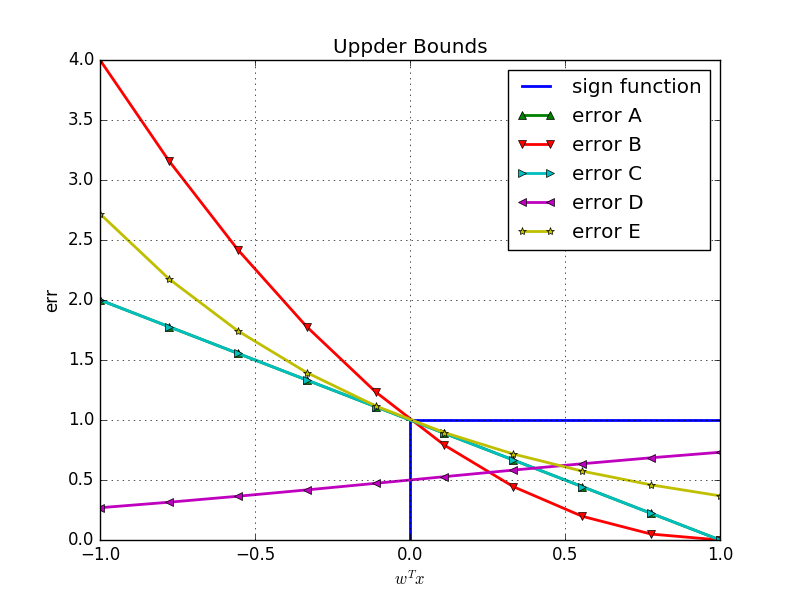
\includegraphics[width=0.8\textwidth]{../results/figure_2.png}
	\caption{Upper Bounds}
\end{figure}
We choose $a$ and $b$ as our upper bounds.
\end{prob}

\begin{prob}{3} - SGD\\
Examine the update rule similar or disimilar with PLA.
\[
    \pdv{E}{w} = \pdv{(max(0, -yw^Tx))}{w} = -yx \text{  if  } yw^Tx > 0
\]
Update rule is 
\[
    w_{t+1} \leftarrow w_t -yx \text{  if  } yw^Tx > 0
\]
Which is not behave like PLA.
\end{prob}

\begin{prob}{4} - GD and Beyond \\
\begin{align*}
    E(u,v) & = e^u + 2e^v + e^{uv} + u^2 -2uv + 2v^2 -3u - 2v \\
    \grad{E} & = (\pdv{E}{u}, \pdv{E}{v}) \\
\end{align*}
where 
\[
    \pdv{E}{u} = e^u + ve^{uv} + 2u -2v -3 \\
    \pdv{E}{v}) = 2e^{2v} + ue^{uv} -2u +4v -2
\]
Then we run the program to see 5 updates
\begin{lstlisting}
python hw_3-4.py
step 1
[ 0.02  0.  ]
step 2
[ 0.03939799  0.0002    ]
step 3
[ 0.05821018  0.00057798]
step 4
[ 0.07645238  0.00111381]
step 5
[ 0.09413996  0.00178911]
\end{lstlisting}
\end{prob}

\begin{prob}{5} - Second order Taylor expansion\\
Expand the error function around $(u,v)$
\[
    E(u+\delta u ,v+\delta v) = \sum_{m,n} \frac{1}{m!n!}\pdv[n]{1}{u}\pdv[m]{1}{v} (u - \delta u)^n (v - \delta v)^m E(u,v)
\]
Up to second order
\[
    E_2 = E(0,0) + E_u\delta u + E_v\delta v + \frac{1}{2}(E_{uu}\delta u^2 + E_{vv}\delta v^2 + 2E_{uv}\delta u \delta v)
\]
each terms are
\begin{align*}
E_u & = e^u + ve^{uv}+2u-2v-3 \\
E_v &= 2e^{2v} ue^{uv} -2u +4v -2\\
E_{uu} &= e^u + v^2e^{uv} + 2 \\
E_{vv} &= 4e^{2v} + u^2e{uv} +4 \\
E_{uv} &= e^{uv} + ue^{uv} -2 
\end{align*}
At the origin
\begin{align*}
b = E(0,0) &= 3 \\
b_u = E_u(0,0) & = -2 \\
b_v = E_v(0,0) &= 0 \\
b_{uu} = E_{uu}(0,0) &= 3 \\
b_{vv} = E_{vv}(0,0) &= 8 \\
b_{uv} = E_{uv}(0,0) &= -1
\end{align*}
\end{prob}

\begin{prob}{6} - Newton Direction\\
We call Newton dircetion \vb{p}, the linear equation follows
\[
    H[E(u,v)]}\vb{p} = - \grad{E(u,v)}
\]
where H is Hessian matrix. It gives
\[
    \vb{p} = - (\grad^2{E(u,v)})^{-1}\grad{E(u,v)}
\]
\end{prob}

\begin{prob}{7} - Newton Updates\\
Run the program to see 5 updates
\begin{lstlisting}
python hw_3-7.py
step 1
(0.07692307692307693, 0.0)
step 2
(0.143561753527925, 0.0029023140091422642)
step 3
(0.20120879953531765, 0.007341944796713773)
step 4
(0.25110373042431666, 0.012467030623187523)
step 5
(0.294360105434023, 0.017763043039507893)
\end{lstlisting}
\end{prob}

\begin{prob}{8} - Regularization and Weight Decay\\
\[
    E_{aug}(w) = E_{in}(w) + \frac{\lambda}{N}\norm{w}^2
\]
Take derivative
\[
    \grad{E_{aug}} = \grad{E_{in}} + \frac{2\lambda}{N}w
\]
The update rule is 
\[
    w_{t+1} \leftarrow w_t - \eta \grad{E_{aug}} = w_t - \eta(\frac{2\lambda}{N}w + \grad{E_{in}})
\]
Simplify as 
\[
    w_{t+1} \leftarrow (1- \frac{2\lambda\eta}{N})w_t - \eta\grad{E_{in}}
\]
\end{prob}

\begin{prob}{9} - Virtual Examples\\
Rewrite loss function in matrix form, better for our analysis
\[
    E(w) = \frac{1}{N+K} ((WX-y)^2 + (W\tilde{X}-\tilde{y})^2)
\]
Then we take derivative and find its optimal solution of $w$, check if it exist.
\[
    0 = \pdv{E}{w} = \frac{2}{N+K} (X^T(wX-y) + \tilde{X}^T(w\tilde{X}-\tilde{y}))
\]
From above equation, we get
\begin{align*}
    (X^TX + \tilde{X}^T\tilde{X})w &= X^Ty + \tilde{X}^T\tilde{y} \\
    w &= (X^TX + \tilde{X}^T\tilde{X})^{-1} X^Ty + \tilde{X}^T\tilde{y}
\end{align*}
\end{prob}

\begin{prob}{10} Ridge regression \\
First, ridge regression loss function is written as 
\[
    E(w) = \frac{\lambda}{N}\norm{w}^2 + \frac{1}{N}\norm{Xw-y}^2
\]
Same technique is applied
\[
    0 = \pdv{E}{w} = \frac{2}{N} (\lambda w + X^TXw -X^Ty)
\]
We get the eqation
\begin{align*}
    (\lambda I + X^TX)w & = X^Ty \\
    w &= (\lambda I + X^TX)^{-1}(X^Ty)
\end{align*}
Then compare to previous result
\begin{align*}
    w_{\text{virtual}} &= (X^TX + \tilde{X}^T\tilde{X})^{-1}( X^Ty + \tilde{X}^T\tilde{y}) \\
    w_{\text{reg}} &= (\lambda I + X^TX)^{-1}(X^Ty)
\end{align*}
Obviously, we choose 
\begin{align*}
    \tilde{X}^T\tilde{X} &= \lambda I \rightarrow \tilde{X} = \sqrt{\lambda} I \\
    \tilde{y}& = 0
\end{align*}
to identify two eqautions.
\end{prob}

\begin{prob}{11} - Experiment with Logistic Regression\\
\begin{lstlisting}
python hw3-11.py
Initialization method: zero
Solver type: vallina
Eout: 0.477000
W=[-0.00385379 -0.18914564  0.26625908 -0.35356593  0.04088776 -0.3794296
  0.01982783  0.33391527 -0.26386754  0.13489328  0.4914191   0.08726107
   -0.25537728 -0.16291797  0.30073678  0.40014954  0.43218808 -0.46227968
     0.43230193 -0.20786372 -0.36936337]
\end{lstlisting}

\end{prob}

\begin{prob}{12} Stochastic Gradient Deschent \\

\begin{lstlisting}
python hw_3-12.py
Initialization method: zero
Solver type: stochastic
Eout: 0.222000
W = [-0.01600468 -0.19177933  0.26585512 -0.36122691  0.05798417 -0.3831994
  0.01821619  0.34271996 -0.2535831   0.11438907  0.50400503  0.08494226
   -0.25182185 -0.17595542  0.31036152  0.40739663  0.43468996 -0.47635182
     0.43959454 -0.19775587 -0.32835603]
\end{lstlisting}
\end{prob}

\begin{prob}{13} Ridge Regression \\
With $\lambda = 1.126$
\begin{lstlisting}
python hw_3-13.py
Initialization method: zero
Ein: 0.035000, Eout: 0.020000
\end{lstlisting}
\[
    E_{in} = 0.035, E_{out} = 0.02
\]
\end{prob}


\begin{prob}{14} Ridge Regression, differenct $\lambda$, minimum $E_{in}$\\
\begin{lstlisting}
python hw_3-14.py
minimum Ein = 0.015000, minimum Eout = 0.015000
lambda with minimum Ein is l=1.0e-10 , Eout=0.02
lambda with minimum Eout is l=1.0e-07 , Ein=0.03
\end{lstlisting}
\begin{figure}[H]
	\centering
	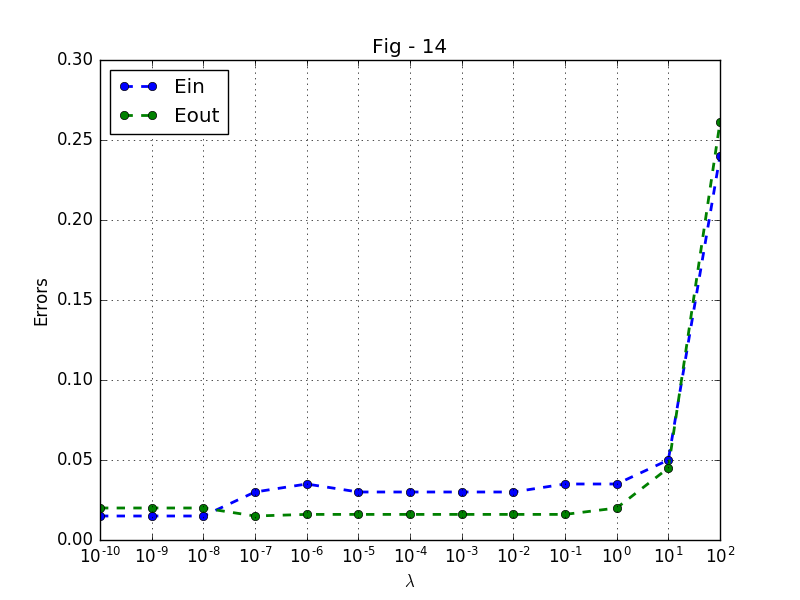
\includegraphics[width=0.8\textwidth]{../results/figure_14.png}
	\caption{Curve of Ein and Eout vs $\lambda$}
\end{figure}
\[
    \lambda = 10^{-10}, E_{in} = 0.015
\]
\end{prob}

\begin{prob}{15} Ridge Regression, differenct $\lambda$, minimum $E_{out}$\\
From above results
\[
    \lambda = 10^{-7}, E_{out} = 0.015
\]
\end{prob}

\begin{prob}{16} Data split, minimum $E_{in}$\\
\begin{lstlisting}
python hw_3-16.py
minimum Ein = 0.000000, minimum Eval = 0.037500 minimum Eout = 0.021000
lambda with minimum Ein is l=1.0e-09 , Eval=0.100000, Eout=0.038000
lambda with minimum Eval is l=1.0e-07 , Ein=0.033333, Eout=0.021000
lambda with minimum Eout is l=1.0e-07 , Ein=0.033333, Eval=0.037500
Run optimal lambda = 1.0e-07 on Dtrain, Ein=0.030000, Eout=0.015000
\end{lstlisting}
\begin{figure}[H]
	\centering
	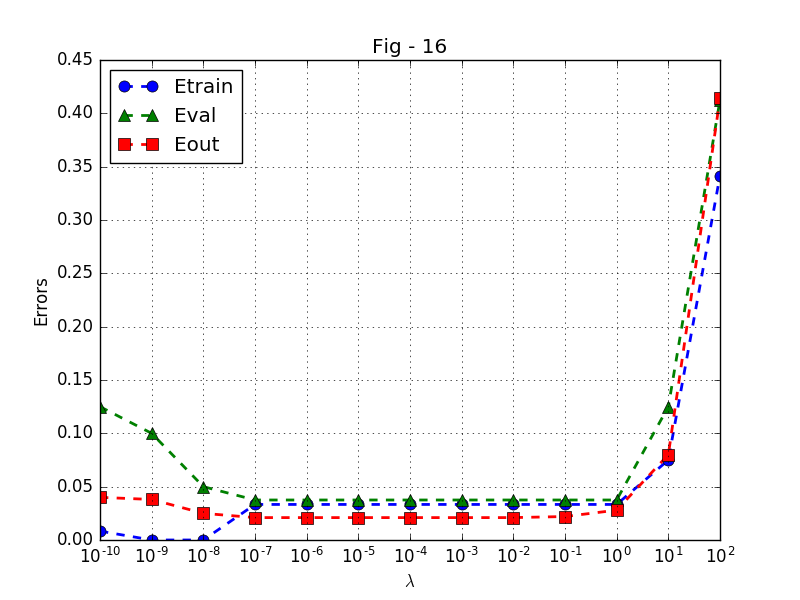
\includegraphics[width=0.8\textwidth]{../results/figure_16.png}
	\caption{Curve of Ein, Eval and Eout vs $\lambda$}
\end{figure}
\[
    \lambda = 10^{-9}, E_{train}(g^-_\lambda) = 0.0, E_{val}(g^-_\lambda) = 0.1, E_{out}(g^-_\lambda) = 0.038
\]
\end{prob}

\begin{prob}{17} Data split, minimum $E_{out}$\\
From above results
\[
    \lambda = 10^{-7}, E_{train}(g^-_\lambda) = 0.0333, E_{val}(g^-_\lambda) = 0.0375, E_{out}(g^-_\lambda) = 0.0375
\]
\end{prob}

\begin{prob}{18} Data split, optimal $\lambda$\\
From above results
\[
    \lambda = 10^{-7}, E_{in}(g^-_\lambda) = 0.03, E_{out}(g^-_\lambda) = 0.015
\]
\end{prob}

\begin{prob}{19} 5-fold cross validation\\
\begin{lstlisting}
python hw_3-19.py
minimum Ecv = 0.030000 minimum Eout = 0.018000
lambda with minimum Ecv is l=1.0e-08 , Eout=0.022
lambda with minimum Eout is l=1.0e-07 , Ecv=0.035
Run optimal lambda = 1.0e-08 on Dtrain, Ein=0.015, Eout=0.02
\end{lstlisting}
\begin{figure}[H]
	\centering
	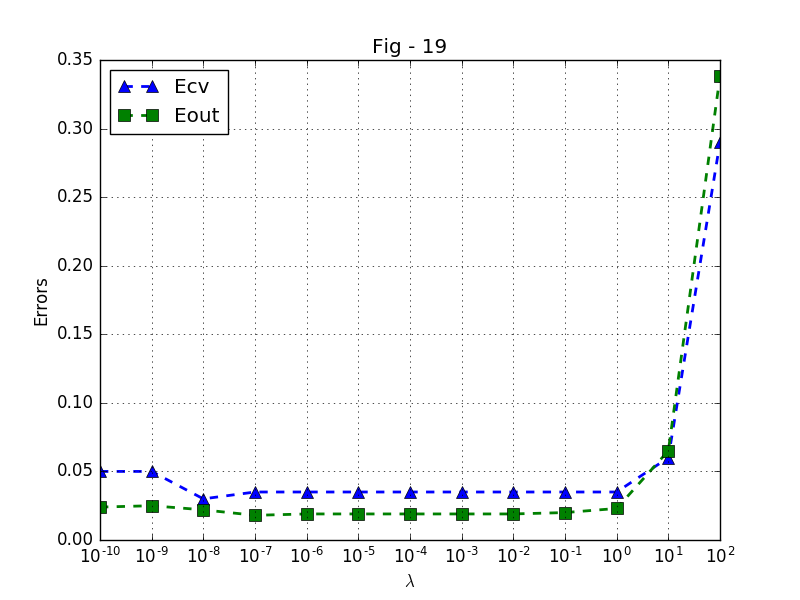
\includegraphics[width=0.8\textwidth]{../results/figure_19.png}
	\caption{Curve of Ecv and Eout vs $\lambda$}
\end{figure}
\[
    \lambda = 10^{-8}, E_{cv-5} = 0.03
\]
\end{prob}

\begin{prob}{20} 5-fold cross validation, optimal\\
From above results
\[
    E_{in}(g_\lambda) = 0.015, E_{out}(g_\lambda) = 0.020
\]
\end{prob}

\begin{prob}{21} Tikhonov regularization\\
Regression loss function is written as 
\[
    E(w) = \frac{1}{N}\norm{\Gamma w}^2 + \frac{1}{N}\norm{Xw-y}^2
\]
Same technique is applied
\[
    0 = \pdv{E}{w} = \frac{2}{N} (\Gamma^T\Gamma w + X^TXw -X^Ty)
\]
We get the eqation
\begin{align*}
    (\Gamma^T\Gamma X^TX)w & = X^Ty \\
    w &= (\Gamma^T\Gamma + X^TX)^{-1}(X^Ty)
\end{align*}
Then compare to previous result
\begin{align*}
    w_{\text{virtual}} &= (X^TX + \tilde{X}^T\tilde{X})^{-1}( X^Ty + \tilde{X}^T\tilde{y}) \\
    w &= (\Gamma^T\Gamma + X^TX)^{-1}(X^Ty)
\end{align*}
We choose 
\begin{align*}
    \tilde{X}^T\tilde{X} &= \Gamma^T\Gamma \rightarrow \tilde{X} = \Gamma \\
    \tilde{y}& = 0
\end{align*}
\end{prob}

\begin{prob}{22} $w_{hint}$ \\
Regression loss function is written as 
\[
    E(w) = \frac{1}{N}\norm{w-w_{hint}}^2 + \frac{1}{N}\norm{Xw-y}^2
\]
Same technique is applied
\[
    0 = \pdv{E}{w} = \frac{2}{N} (w - w_{hint}+ X^TXw -X^Ty)
\]
We get the eqation
\begin{align*}
    w &= (I + X^TX)^{-1}(X^Ty + w_{hint})
\end{align*}
Then compare to previous result
\begin{align*}
    w_{\text{virtual}} &= (X^TX + \tilde{X}^T\tilde{X})^{-1}( X^Ty + \tilde{X}^T\tilde{y}) \\
    w &= (I + X^TX)^{-1}(X^Ty + w_{hint})
\end{align*}
We choose 
\begin{align*}
    \tilde{X}^T\tilde{X} &= I = \tilde{X} \\
    \tilde{y}& = w_{hint}
\end{align*}
\end{prob}
\end{CJK} 
\end{document}